\documentclass{standalone}
\usepackage{tikz}
\usetikzlibrary{patterns, positioning}
\usepackage[sfdefault]{ClearSans} %% option 'sfdefault' activates Clear Sans as the default text font
\usepackage[T1]{fontenc}

\begin{document}
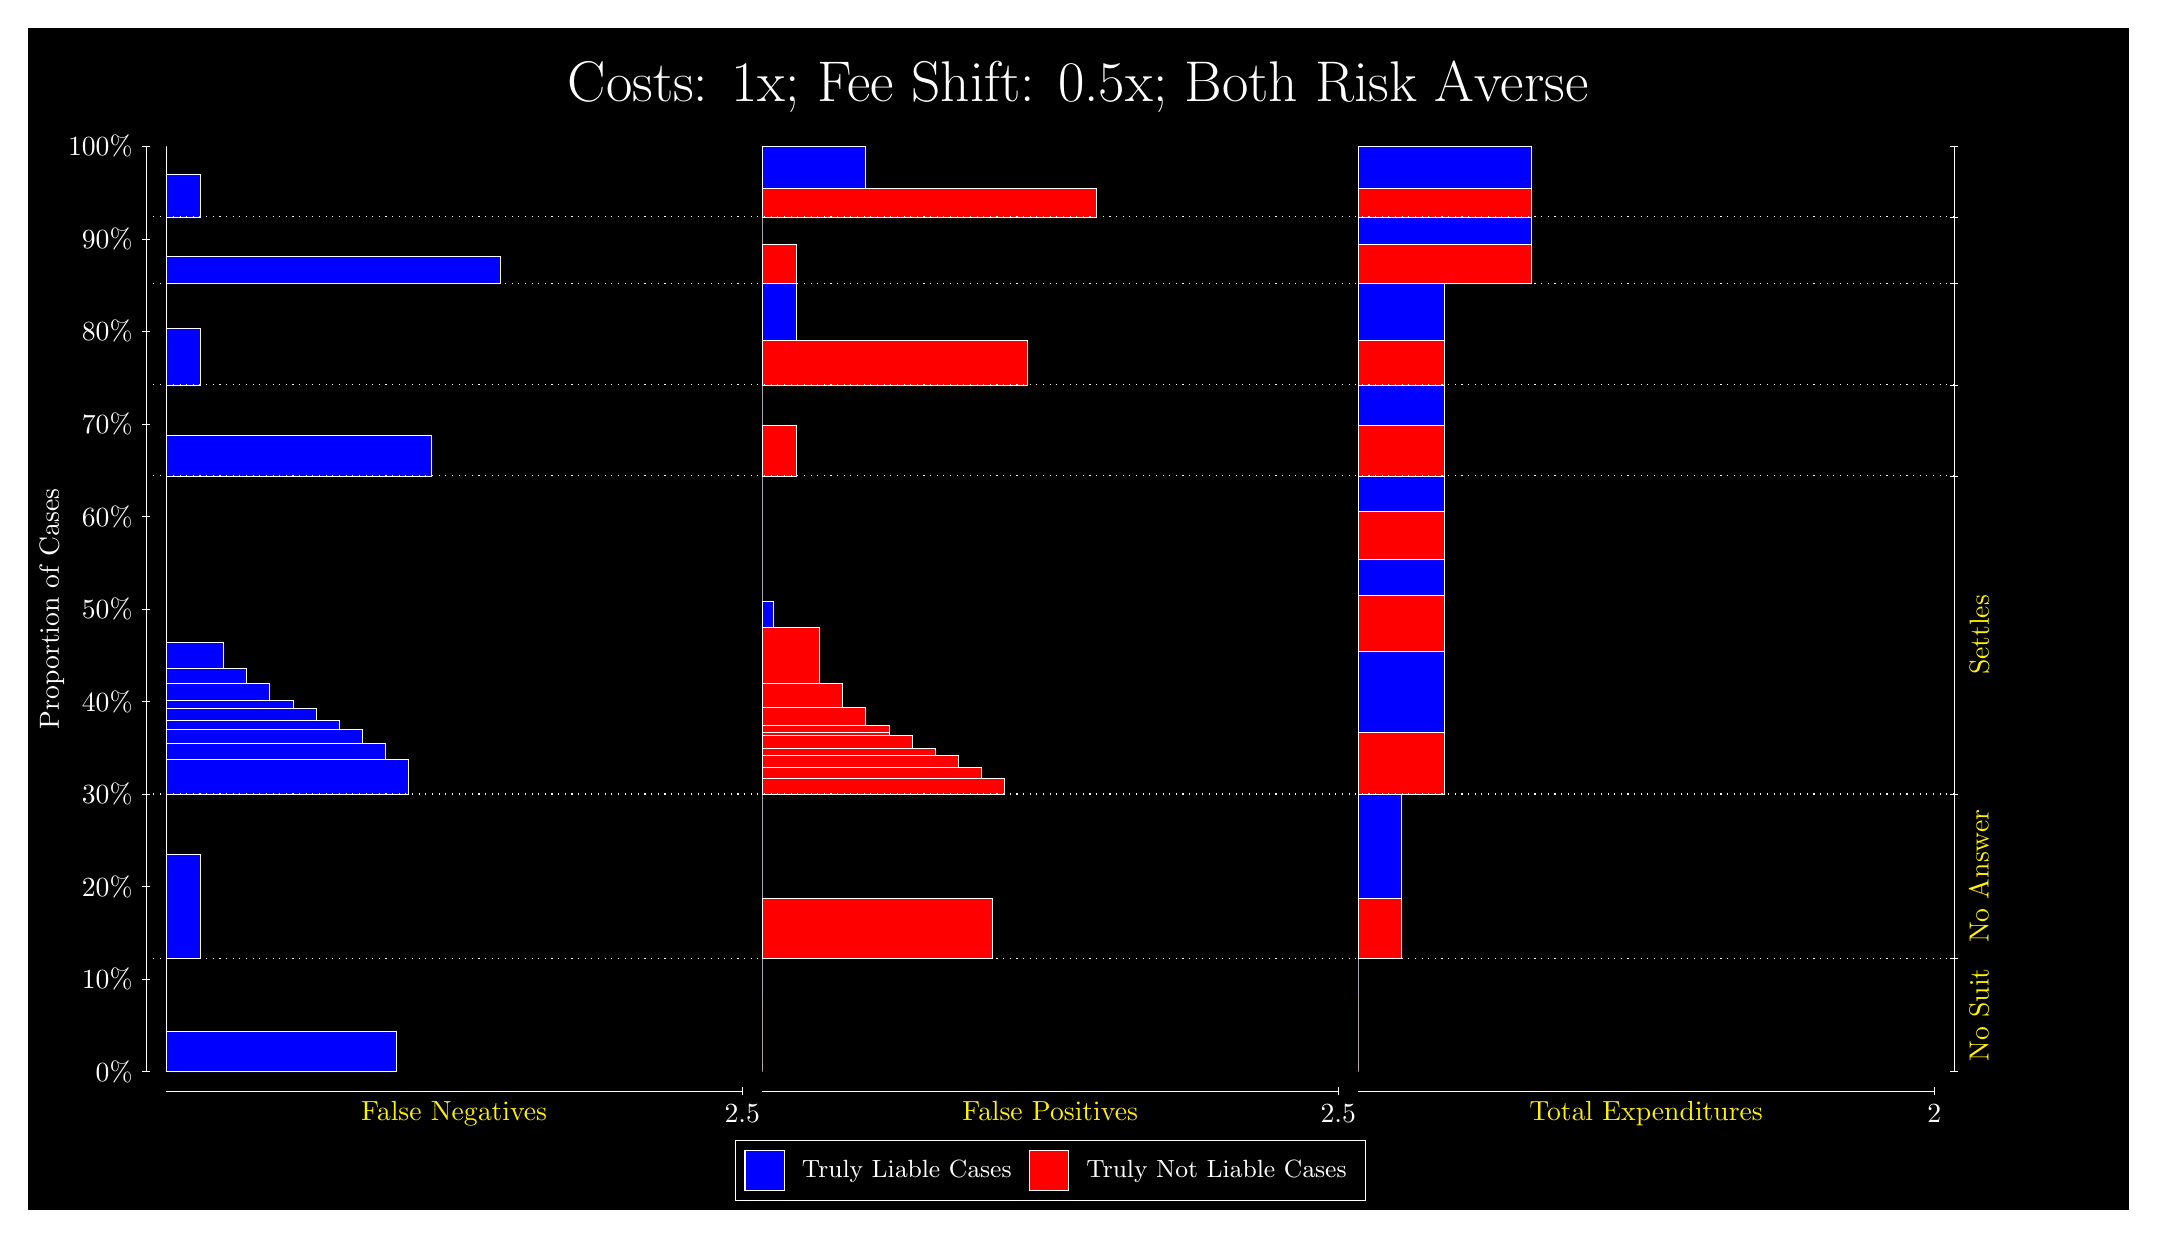
\begin{tikzpicture}
\draw[fill=black] (0,0) rectangle (26.667,15);
\draw[text=white] (0,13.5) rectangle (26.667,15) node[midway] {\huge Costs: 1x; Fee Shift: 0.5x; Both Risk Averse};
\draw[white, very thin] (1.5,1.75) -- (1.5,13.5);
\node[rotate=90, text=white, anchor=center] at (0.3, 7.625) {Proportion of Cases};
\draw[white, very thin] (1.45,1.75) -- (1.55,1.75);
\node[text=white, anchor=east] at (1.45, 1.75) {0\%};
\draw[white, very thin] (1.45,2.925) -- (1.55,2.925);
\node[text=white, anchor=east] at (1.45, 2.925) {10\%};
\draw[white, very thin] (1.45,4.1) -- (1.55,4.1);
\node[text=white, anchor=east] at (1.45, 4.1) {20\%};
\draw[white, very thin] (1.45,5.275) -- (1.55,5.275);
\node[text=white, anchor=east] at (1.45, 5.275) {30\%};
\draw[white, very thin] (1.45,6.45) -- (1.55,6.45);
\node[text=white, anchor=east] at (1.45, 6.45) {40\%};
\draw[white, very thin] (1.45,7.625) -- (1.55,7.625);
\node[text=white, anchor=east] at (1.45, 7.625) {50\%};
\draw[white, very thin] (1.45,8.8) -- (1.55,8.8);
\node[text=white, anchor=east] at (1.45, 8.8) {60\%};
\draw[white, very thin] (1.45,9.975) -- (1.55,9.975);
\node[text=white, anchor=east] at (1.45, 9.975) {70\%};
\draw[white, very thin] (1.45,11.15) -- (1.55,11.15);
\node[text=white, anchor=east] at (1.45, 11.15) {80\%};
\draw[white, very thin] (1.45,12.325) -- (1.55,12.325);
\node[text=white, anchor=east] at (1.45, 12.325) {90\%};
\draw[white, very thin] (1.45,13.5) -- (1.55,13.5);
\node[text=white, anchor=east] at (1.45, 13.5) {100\%};

\draw[white, very thin] (24.457,1.75) -- (24.457,13.5);
\draw[white, very thin] (24.407,1.75) -- (24.507,1.75);
\node[anchor=west] at (24.407, 1.75) {};
\draw[white, very thin] (24.407,3.1862) -- (24.507,3.1862);
\node[anchor=west] at (24.407, 3.1862) {};
\draw[white, very thin] (24.407,5.274) -- (24.507,5.274);
\node[anchor=west] at (24.407, 5.274) {};
\draw[white, very thin] (24.407,9.3155) -- (24.507,9.3155);
\node[anchor=west] at (24.407, 9.3155) {};
\draw[white, very thin] (24.407,10.471) -- (24.507,10.471);
\node[anchor=west] at (24.407, 10.471) {};
\draw[white, very thin] (24.407,11.762) -- (24.507,11.762);
\node[anchor=west] at (24.407, 11.762) {};
\draw[white, very thin] (24.407,12.605) -- (24.507,12.605);
\node[anchor=west] at (24.407, 12.605) {};
\draw[white, very thin] (24.407,13.5) -- (24.507,13.5);
\node[anchor=west] at (24.407, 13.5) {};

\draw[white, very thin, fill=blue] (1.75,1.75) rectangle (4.6775,2.2561);
\draw[white, very thin, fill=red] (1.75,2.2561) rectangle (1.75,3.1862);
\draw[white, very thin, fill=blue] (1.75,3.1862) rectangle (2.1891,4.5067);
\draw[white, very thin, fill=red] (1.75,4.5067) rectangle (1.75,5.274);
\draw[white, very thin, fill=blue] (1.75,5.274) rectangle (4.8239,5.7203);
\draw[white, very thin, fill=blue] (1.75,5.7203) rectangle (4.5312,5.9222);
\draw[white, very thin, fill=blue] (1.75,5.9222) rectangle (4.2384,6.0958);
\draw[white, very thin, fill=blue] (1.75,6.0958) rectangle (3.9457,6.2099);
\draw[white, very thin, fill=blue] (1.75,6.2099) rectangle (3.6529,6.3685);
\draw[white, very thin, fill=blue] (1.75,6.3685) rectangle (3.3602,6.4586);
\draw[white, very thin, fill=blue] (1.75,6.4586) rectangle (3.0674,6.6759);
\draw[white, very thin, fill=blue] (1.75,6.6759) rectangle (2.7746,6.8724);
\draw[white, very thin, fill=blue] (1.75,6.8724) rectangle (2.4819,7.203);
\draw[white, very thin, fill=red] (1.75,7.203) rectangle (1.75,9.3155);
\draw[white, very thin, fill=blue] (1.75,9.3155) rectangle (5.1167,9.834);
\draw[white, very thin, fill=red] (1.75,9.834) rectangle (1.75,10.471);
\draw[white, very thin, fill=blue] (1.75,10.471) rectangle (2.1891,11.193);
\draw[white, very thin, fill=red] (1.75,11.193) rectangle (1.75,11.762);
\draw[white, very thin, fill=blue] (1.75,11.762) rectangle (5.9949,12.105);
\draw[white, very thin, fill=red] (1.75,12.105) rectangle (1.75,12.605);
\draw[white, very thin, fill=blue] (1.75,12.605) rectangle (2.1891,13.14);
\draw[white, very thin, fill=red] (1.75,13.14) rectangle (1.75,13.5);
\draw[white, very thin, fill=red] (9.3189,1.75) rectangle (9.3189,2.6801);
\draw[white, very thin, fill=blue] (9.3189,2.6801) rectangle (9.3189,3.1862);
\draw[white, very thin, fill=red] (9.3189,3.1862) rectangle (12.246,3.9535);
\draw[white, very thin, fill=blue] (9.3189,3.9535) rectangle (9.3189,5.274);
\draw[white, very thin, fill=red] (9.3189,5.274) rectangle (12.393,5.4778);
\draw[white, very thin, fill=red] (9.3189,5.4778) rectangle (12.1,5.6133);
\draw[white, very thin, fill=red] (9.3189,5.6133) rectangle (11.807,5.7718);
\draw[white, very thin, fill=red] (9.3189,5.7718) rectangle (11.515,5.8546);
\draw[white, very thin, fill=red] (9.3189,5.8546) rectangle (11.222,6.0162);
\draw[white, very thin, fill=red] (9.3189,6.0162) rectangle (10.929,6.0598);
\draw[white, very thin, fill=red] (9.3189,6.0598) rectangle (10.929,6.1418);
\draw[white, very thin, fill=red] (9.3189,6.1418) rectangle (10.636,6.3743);
\draw[white, very thin, fill=red] (9.3189,6.3743) rectangle (10.344,6.6748);
\draw[white, very thin, fill=red] (9.3189,6.6748) rectangle (10.051,7.3864);
\draw[white, very thin, fill=blue] (9.3189,7.3864) rectangle (9.4652,7.7171);
\draw[white, very thin, fill=blue] (9.3189,7.7171) rectangle (9.3189,9.3155);
\draw[white, very thin, fill=red] (9.3189,9.3155) rectangle (9.758,9.9528);
\draw[white, very thin, fill=blue] (9.3189,9.9528) rectangle (9.3189,10.471);
\draw[white, very thin, fill=red] (9.3189,10.471) rectangle (12.686,11.04);
\draw[white, very thin, fill=blue] (9.3189,11.04) rectangle (9.758,11.762);
\draw[white, very thin, fill=red] (9.3189,11.762) rectangle (9.758,12.262);
\draw[white, very thin, fill=blue] (9.3189,12.262) rectangle (9.3189,12.605);
\draw[white, very thin, fill=red] (9.3189,12.605) rectangle (13.564,12.964);
\draw[white, very thin, fill=blue] (9.3189,12.964) rectangle (10.636,13.5);
\draw[white, very thin, fill=red] (16.888,1.75) rectangle (16.888,2.6801);
\draw[white, very thin, fill=blue] (16.888,2.6801) rectangle (16.888,3.1862);
\draw[white, very thin, fill=red] (16.888,3.1862) rectangle (17.437,3.9535);
\draw[white, very thin, fill=blue] (16.888,3.9535) rectangle (17.437,5.274);
\draw[white, very thin, fill=red] (16.888,5.274) rectangle (17.986,6.0598);
\draw[white, very thin, fill=blue] (16.888,6.0598) rectangle (17.986,7.0916);
\draw[white, very thin, fill=red] (16.888,7.0916) rectangle (17.986,7.8032);
\draw[white, very thin, fill=blue] (16.888,7.8032) rectangle (17.986,8.2496);
\draw[white, very thin, fill=red] (16.888,8.2496) rectangle (17.986,8.8646);
\draw[white, very thin, fill=blue] (16.888,8.8646) rectangle (17.986,9.3155);
\draw[white, very thin, fill=red] (16.888,9.3155) rectangle (17.986,9.9528);
\draw[white, very thin, fill=blue] (16.888,9.9528) rectangle (17.986,10.471);
\draw[white, very thin, fill=red] (16.888,10.471) rectangle (17.986,11.04);
\draw[white, very thin, fill=blue] (16.888,11.04) rectangle (17.986,11.762);
\draw[white, very thin, fill=red] (16.888,11.762) rectangle (19.083,12.262);
\draw[white, very thin, fill=blue] (16.888,12.262) rectangle (19.083,12.605);
\draw[white, very thin, fill=red] (16.888,12.605) rectangle (19.083,12.964);
\draw[white, very thin, fill=blue] (16.888,12.964) rectangle (19.083,13.5);
\draw[white, dotted] (1.5,3.1862) -- (24.457,3.1862);
\draw[white, dotted] (1.5,5.274) -- (24.457,5.274);
\draw[white, dotted] (1.5,9.3155) -- (24.457,9.3155);
\draw[white, dotted] (1.5,10.471) -- (24.457,10.471);
\draw[white, dotted] (1.5,11.762) -- (24.457,11.762);
\draw[white, dotted] (1.5,12.605) -- (24.457,12.605);
\draw[white, very thin] (1.75,1.5) -- (9.0689,1.5);
\node[text=yellow, anchor=north] at (5.4094, 1.5) {False Negatives};
\draw[white, very thin] (9.0689,1.45) -- (9.0689,1.55);
\node[text=white, anchor=north] at (9.0689, 1.45) {2.5};

\draw[white, very thin] (9.3189,1.5) -- (16.638,1.5);
\node[text=yellow, anchor=north] at (12.978, 1.5) {False Positives};
\draw[white, very thin] (16.638,1.45) -- (16.638,1.55);
\node[text=white, anchor=north] at (16.638, 1.45) {2.5};

\draw[white, very thin] (16.888,1.5) -- (24.207,1.5);
\node[text=yellow, anchor=north] at (20.547, 1.5) {Total Expenditures};
\draw[white, very thin] (24.207,1.45) -- (24.207,1.55);
\node[text=white, anchor=north] at (24.207, 1.45) {2};

\node[text=yellow, centered, rotate=90] at (24.777, 2.4681) {No Suit};
\node[text=yellow, centered, rotate=90] at (24.777, 4.2301) {No Answer};
\node[text=yellow, centered, rotate=90] at (24.777, 7.2947) {Settles};





\draw (12.978300999999998,1.5) node[draw=none] (baseCoordinate) {};
\begin{scope}[align=center]
        \matrix[scale=0.5, draw=white, below=0.5cm of baseCoordinate, nodes={draw}, column sep=0.1cm]{
            \node[rectangle, draw, minimum width=0.5cm, minimum height=0.5cm, fill=blue] {}; &
            \node[draw=none, font=\small, text=white] (B) {Truly Liable Cases}; &
            \node[rectangle, draw, minimum width=0.5cm, minimum height=0.5cm, fill=red] {}; &
            \node[draw=none, font=\small, text=white] (B) {Truly Not Liable Cases}; \\
            };
\end{scope}

\end{tikzpicture}
\end{document}